\section{Background: Trace\textit{a} and SysML}\label{sec:background}
\sideboxbegin{o}
This section introduces existing techniques we build upon (SysML and Trace\textit{a}) then presents high level requirements for trustable traceability.
\sideboxend

% Nous avons développé Trace\textit{a} pour combler les limitations éprouvées par les langages dédiés à la traçabilité. Dans la littérature spécialisée, les \textit{traces} et leurs éléments atomiques, les \textit{liens}, sont considérés comme des éléments dont la qualité n'est jamais remise en question.
% \ughu{Les liens sont cependant volatiles: dû à la volatilité des systèmes logiciels, mais aussi à l'utilisation grandissante de techniques non-déterministes pour l'identification des liens. }

% Avec la recrudescence de l'utilisation du traçage (due à l'implication toujours plus intrusive des logiciels dans notre quotidien et dans nos industries), garantir le niveau de confiance dans les traces devient primordial. Aucune étude considérée lors de notre premier livrable ne prenait en compte cet aspect.

% \ughu{Cette utilisation, guidée par l'édification de standard de qualité, doit permettre la certification de modules logiciels pour faire la jonction avec les besoin législatifs grandissants. }



This section first introduces the Trace\textit{a} metamodel \cite{batot2021-not-another-metamodel} and presents in particular the functionalities for evaluating the confidence of trace links.   

Then, an introduction to the KerML / SysMLv2 architecture establishes the preliminary notions necessary for understanding the project. The use of SysML does not require special knowledge of KerML (according to the SysML v2 Submission Team (SST)). However, it seems reductive to understand a language without addressing its foundations. We will see how the integration of Trace\textit{a} can and should also be considered at the KerML level.
Finally this section describes the high level requirements for quality traceability as defined in previous deliverables.

% Le métamodèle Tracea a été développé pour pallier aux limitations des langages (et autres modélisations) de la traçabilité pour le logiciel.

\subsection{Existing}
\subsubsection{Trace\textit{a}}
\begin{figure}[ht]     
	\centering
	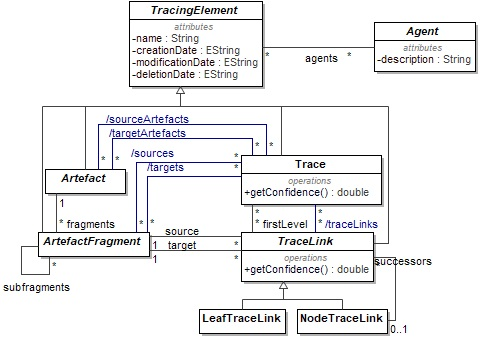
\includegraphics[width=.8\linewidth]{images/core.jpg}
	\caption{Core of Trace\textit{a}: Artefacts and (Trace)Links.}
	\label{fig:mm-core}
\end{figure}


\Fig{fig:mm-core} presents the core of the Trace\textit{a} language. At its center we find the notions of \textit{Trace}, \textit{link} (TraceLink), \textit{artefact} and \textit{fragment}. Links make up the traces and connect \textit{fragments} of the system to each other. We also notice the abstract nature of the Artefacts and Fragments. These are by definition volatile and must be redefined for each project or company to be best suited to concrete tracing needs.

\Fig{fig:mm-explainability} shows an extract from Trace\textit{a} specialized in the qualification of traces and links. The concepts of confidence (applied to Trace and TraceLink), as well as the creation, modification and deletion dates of the trace elements are present. These concepts make it possible to put in contact the evolution of the elements, their agent in charge (human or not) and the level of confidence linked to the traces and links. 

\begin{figure}[h]     
	\centering
	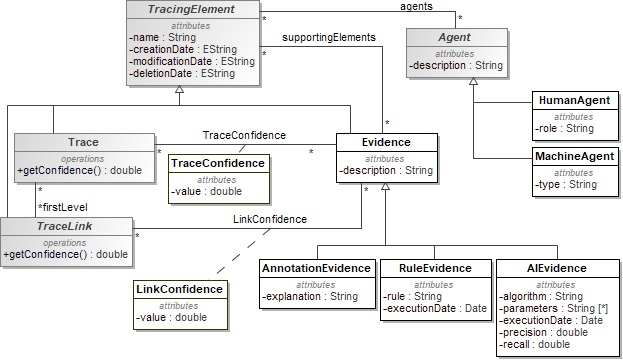
\includegraphics[width=.8\linewidth]{images/explainability.jpg}
	\caption{Excerpt of Trace\textit{a} dedicated to the quality of trace and link.}
	\label{fig:mm-explainability}
\end{figure}

Moreover, Trace\textit{a} allows the attribution to the traces of information (evidences) allowing their confidence values to be justified. Depending on the nature of the means of identification employed, these are an identification rule, a simple textual annotation, or the details of the training configuration and execution of a learning algorithm (classes at the bottom right corner). The execution parameters of the automated identification means (rules or learning algorithms) are thus available for consultation after their execution. The evidence may also point to supporting elements implicated in the calculation and justification of the level of confidence.


% \begin{figure}[h]     
% 	\centering
% 	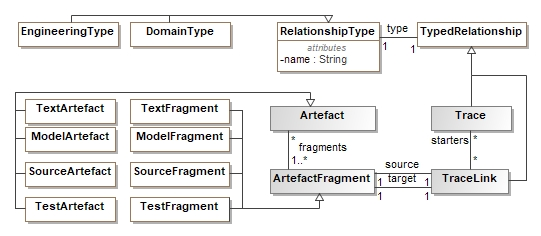
\includegraphics[width=.7\linewidth]{images/customization.jpg}
% 	\caption{Excerpt of Trace\textit{a} dedicated to the customization of traces and links.}
% 	\label{fig:mm-custom}
% \end{figure}




\subsubsection{The KerML/SysMLv2 ecosystem.}
\Fig{fig:kermlsysml} shows the architecture of the KerML / SysML ecosystem. The Kernel Modeling Language (KerML) formally defines a set of concepts allowing the development of languages specific to a given activity. 
% It is derived from three main classes: elements (Element), links (Relationship) and annotations (Annotation). These classes form the \textit{root} elements of the language (Root syntax) and are purely syntactic: they have no semantics related to modeling. These are linguistic elements allowing the construction of complex structures.
KerML has language elements defined at the syntax core level, themselves reusing the root language elements to allow the use of constructs specific to system modeling. These classes are redefined to establish the precise elements of modeling: relative to the construction of sequence diagrams, classes, activity, and the whole panoply of UML diagrams, among others. (For more details, see the KerML metamodel specification document ~\cite{kerML}).

\begin{figure}[ht]     
	\centering
	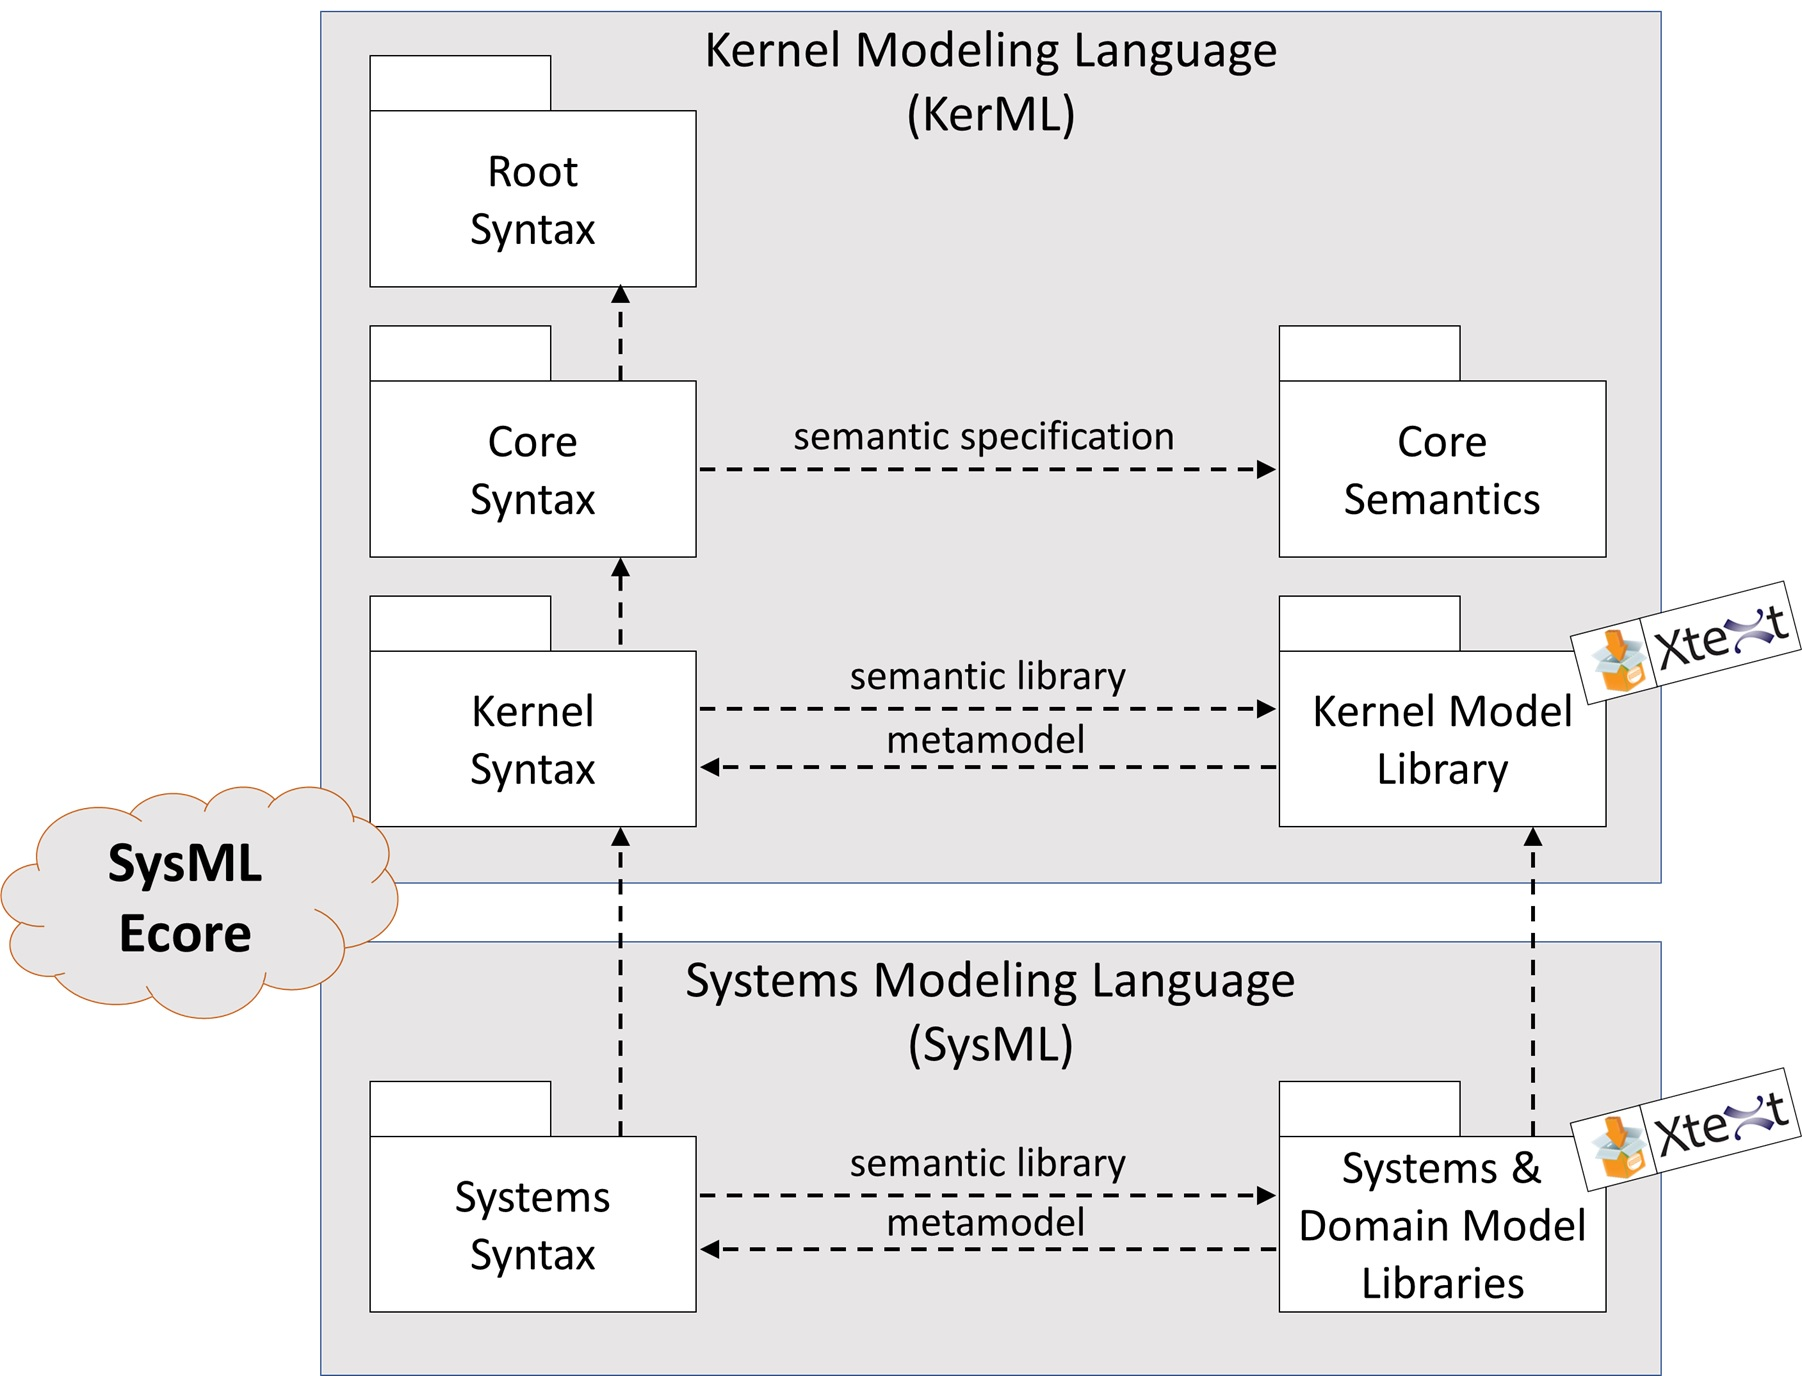
\includegraphics[width=.8\linewidth]{images/KerMLSysML.jpg}
	\caption{The KerML/SysMLv2 ecosystem.}
	\label{fig:kermlsysml}
\end{figure}



As shown in \Fig{fig:sysml}, the SysML language is constructed as an extension of the KerML Kernel metamodel ~\cite{kerML}. The SysML abstract syntax reuses the abstract kernel syntax, providing specialized constructs for modeling systems. Additionally, the SysML System Model Library extends the Kernel Model Library to provide the semantic specification for SysML. Finally, SysML provides an additional set of domain libraries to provide a rich set of reference models in various areas important for systems modeling (such as quantities and units, and basic geometry). (SysML p.69~\cite{sysml})

Finally, it is important to note that concrete elements of KerML cannot be instantiated from SysML.

\begin{figure}[ht]     
	\centering
	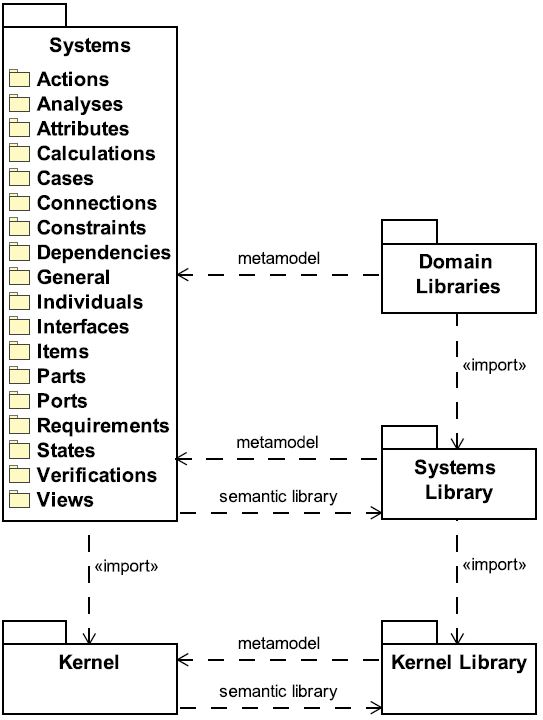
\includegraphics[width=.5\linewidth]{images/sysml.JPG}
	\caption{Architecture de SysML.}
	\label{fig:sysml}
\end{figure}

% \textit{\ugh{"}The Root layer is purely syntactic and has no modeling semantics. The Core is grounded in mathematical semantics (based on 7.3.1.2), supported by the Base package from the Kernel Model Library (see 8.2). The Kernel layer is given semantics fully through its relationship to the Model Library (see Clause 8). The semantic specification for each Kernel sub-package summarizes constraints on Kernel abstract syntax elements that specify how the model library is used when models are constructed following the abstract syntax.\ugh{"} (KerML p. 26)}

% \ughu{The [kerML] specification includes a metamodel that defines how models are structured (syntax) and model libraries that specify how real or virtual things are constructed or operated according to those models (semantics)~\cite{kerML}}.

% \begin{descriptioncompact}
%     \item[1 - KerML] Formal description of language elements
%     \item[2 - SysML] Adaptation to system development
% \end{descriptioncompact}

\subsubsection{Elements, Relationships, and Annotations}
KerML is organized around three fundamental concepts: Elements, Relationships and Annotations. The first two form the structure of the language and the third allows an orthogonal approach to it. Every element in SysML derives from these concepts.

\begin{figure}[ht]     
	\centering
	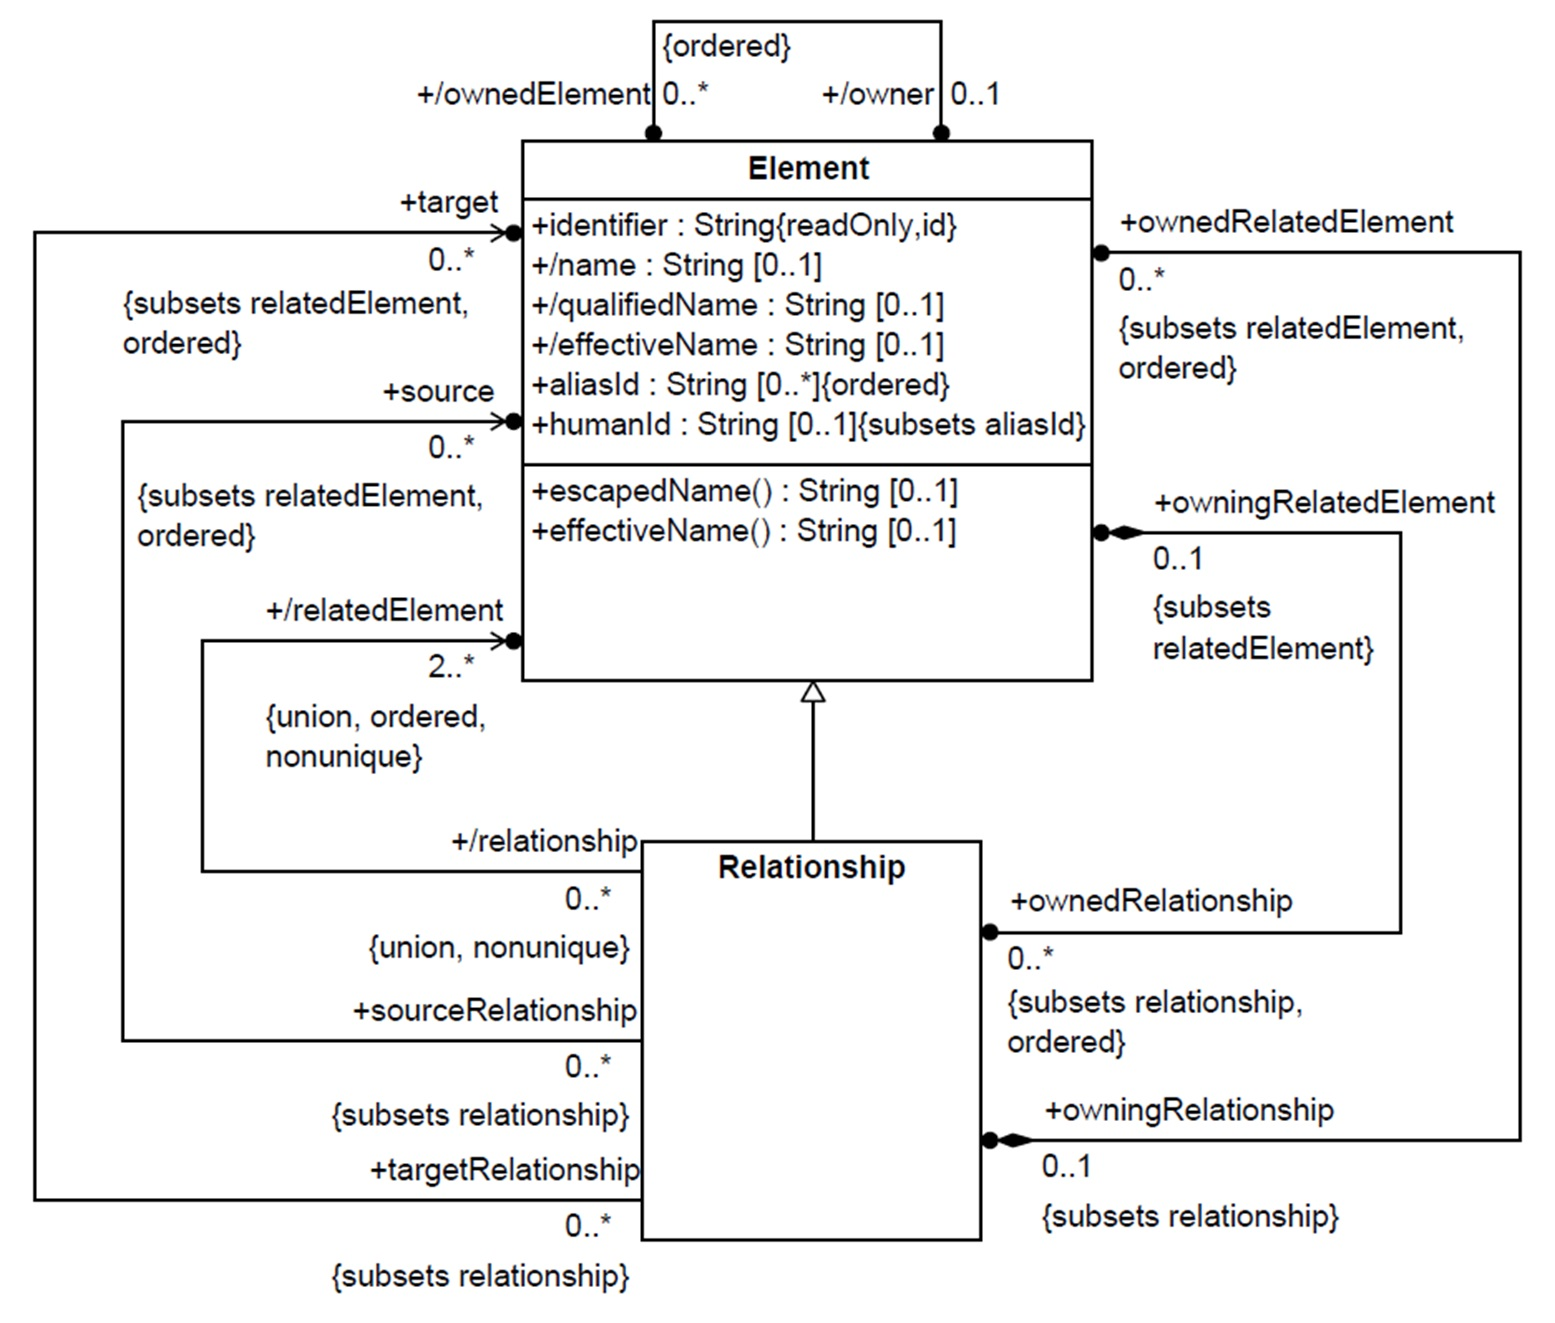
\includegraphics[width=.8\linewidth]{images/elementrelationship.jpg}
	\caption{Elements et Relationships dans KerML.}
	\label{fig:eltrel}
\end{figure}
More precisely, KerML makes it possible to represent complex structures in the form of graphs in which the nodes are Elements and the arcs are Relationships. Since a Relationship is itself an Element, relationship chains are also authorized and allow the nesting of features (\textit{nested features}). \Fig{fig:eltrel} specifies the links that exist between Element and Relationship. The \textit{ownership} is not detailed in this document but deserves to be mentioned here. Every Element is \textit{owned} by another. When one element is deleted, all the elements it \textit{owns} are also deleted.
For information purposes, Figures~\ref{fig:eltshierarchy} and~\ref{fig:relhierarchy} show the hierarchy derived from Elements and Relationships in KerML.

\begin{figure}[ht]     
	\centering
	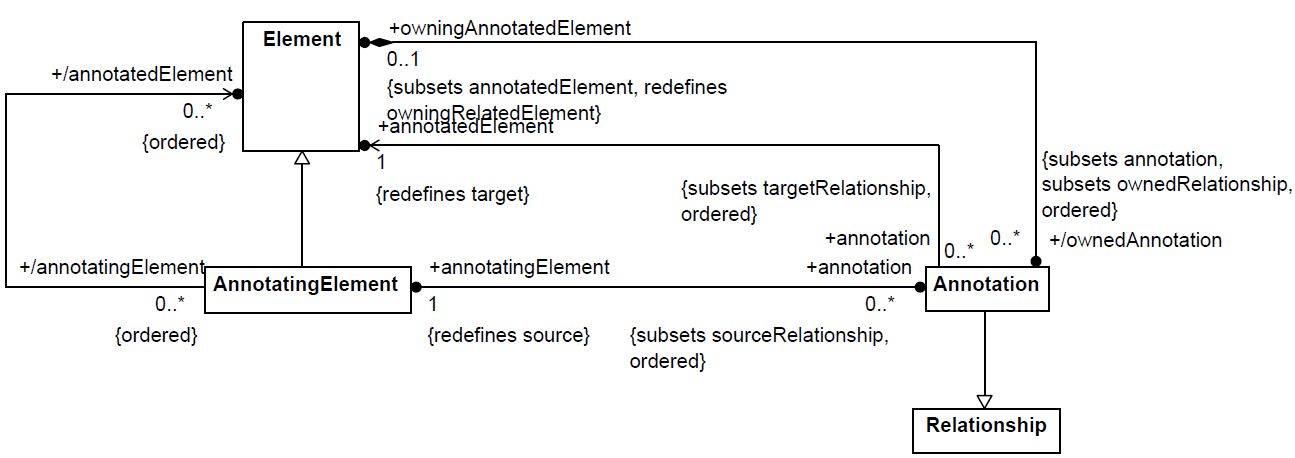
\includegraphics[width=.99\linewidth]{images/annotations.JPG}
	\caption{Annotations in KerML.}
	\label{fig:annot}
\end{figure}

On the other hand, "an Annotation is a relationship between an element and an AnnotatingElement that provides additional information about the annotated element. Each annotation falls between a single AnnotatingElement and a single element being annotated, but an AnnotatingElement can have multiple annotation relationships with different annotatedElements, and any element can have multiple annotations." (KerML Specification, p. 37~\cite{kerML}).

In the case of traceability, annotations can be used to identify types of links and tag \textit{relevant} links (\textit{i.e.,} according to the specific use we want to make of them). We will speak of an \textit{orthogonal} approach by annotations. 
\vspace{5em}
\begin{figure}[ht]     
	\centering
	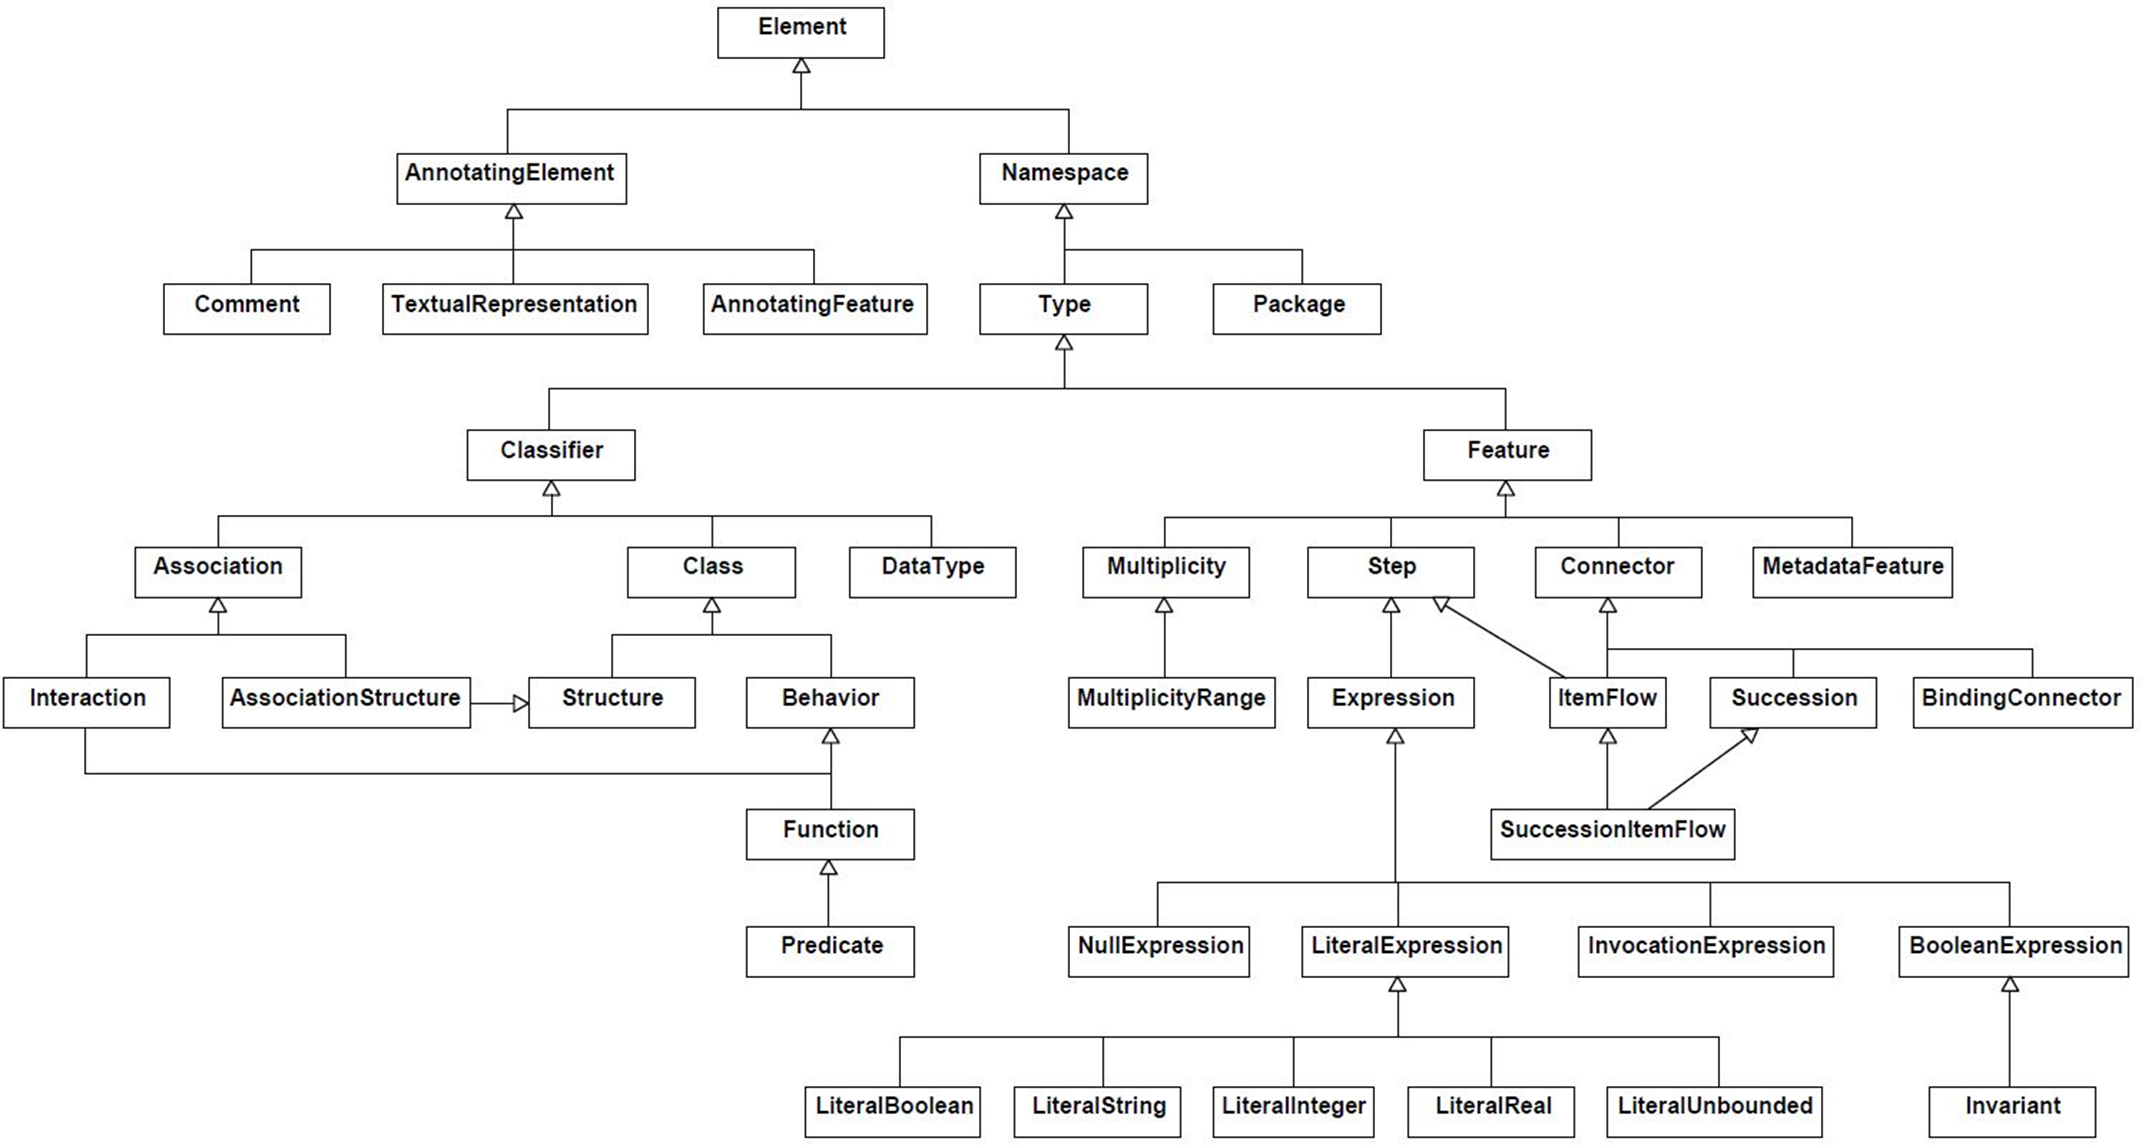
\includegraphics[width=.99\linewidth]{images/kerml-element.png}
	\caption{Hierarchy of KerML Elements.}
	\label{fig:eltshierarchy}
\end{figure}

\begin{figure}[ht]     
	\centering
	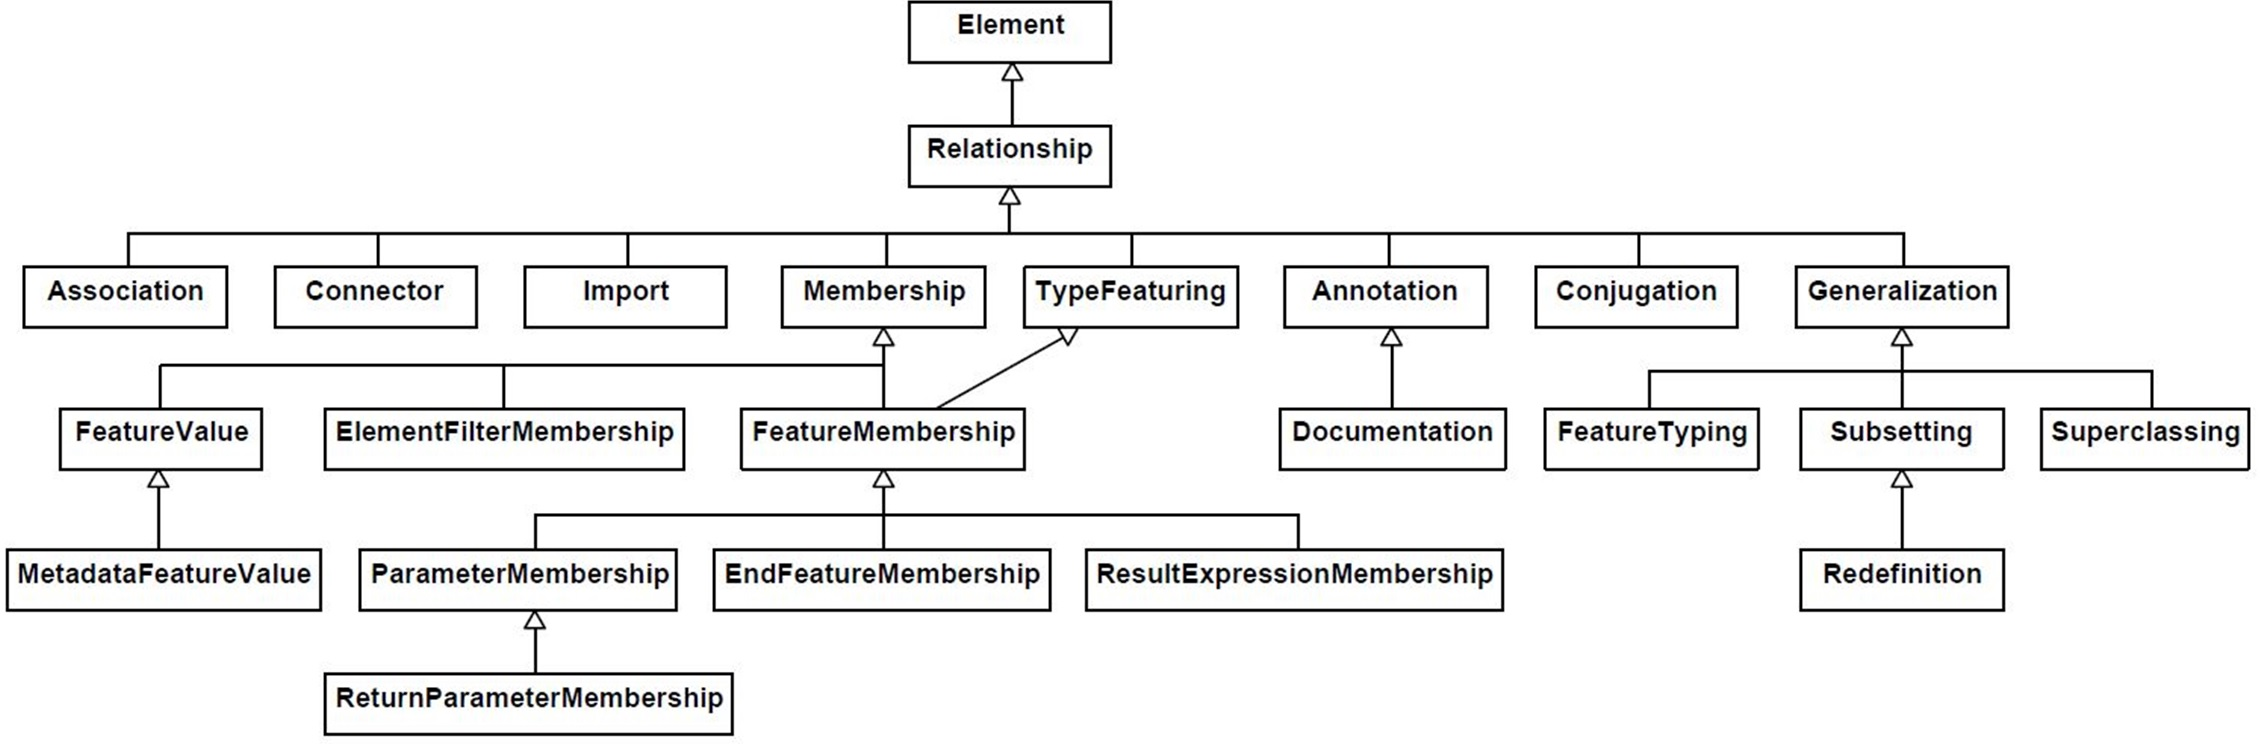
\includegraphics[width=.99\linewidth]{images/kerml-relationship.jpg}
	\caption{Hierarchy of KerML Relationships.}
	\label{fig:relhierarchy}
\end{figure}


% \begin{descriptioncompact}
%     \item[Elements] Top level (root) element of the KerML language.
%     \item[Relationships] Links between elements.
%     \item[Annotations] Open window to orthogonal considerations.
% \end{descriptioncompact}


\subsection{Goals}
The needs in terms of traceability have been established in Deliverable 1 ~ \ cite {deliverable1}. We summarize here the high level needs to satisfy a quality traceability, \textit{i.e.,} allowing to qualify quantitatively and qualitatively the identified links useful for the tracing.
    
\subsubsection{Mastering complexity}
The tracing must allow to measure or approximate the complexity of the system. Since the concept of "Complexity" suffers from a high degree of volatility, its measurement (or its \textit{proxy}) requires a consequent adaptability.
    
\subsubsection{Increase the ability to scale the system}
To facilitate the monitoring of the evolution of the system over time, tracing makes it possible to concentrate the measurement of the impact (\textit{eg,} of a change) on (types of) specifically chosen links.
    % \ item [Independence from target system]
    
\subsubsection{Maintain a degree of independence from the target system}
Tracing must not influence the system. It must remain independent, or \textit{orthogonal}, so that \textit{i)} it does not alter the evolution of the system, \textit{ii)} it does not depend on decisions relating to the development of the system, and \textit{iii)} it remains possible to plot systems of systems (\textit{ie,} written in different languages, on different platforms).% \end{descriptioncompact}

